\subsubsubsection{Bootstrap}
In order to neatly start the application layer, we have to consider the
dependencies among the entity types exposed in \ref{fig:sd-entity-types-deps}.
Moreover we have to take into account that this layer can not decide by itself
when it is time to boot, because this is ruled by the middleware.
The bootstrap of the application layer needs a \textit{Master} process,
which has to create the entities based on the configuration provided by
the middleware layer.

Bearing in mind the aforementioned dependencies:
\begin{itemize}
  \item \textit{Reactive} entities have to start before \textit{active}
ones, because the latter use the former;
  \item \textit{Passive} entities have no particular dependency. Since
they are stateless and they logically belong to \textit{reactive} entities
(e.g. road signs belong to roads), they have to be instantiated along with them.
\end{itemize}

\begin{figure}[H]
  \centering
  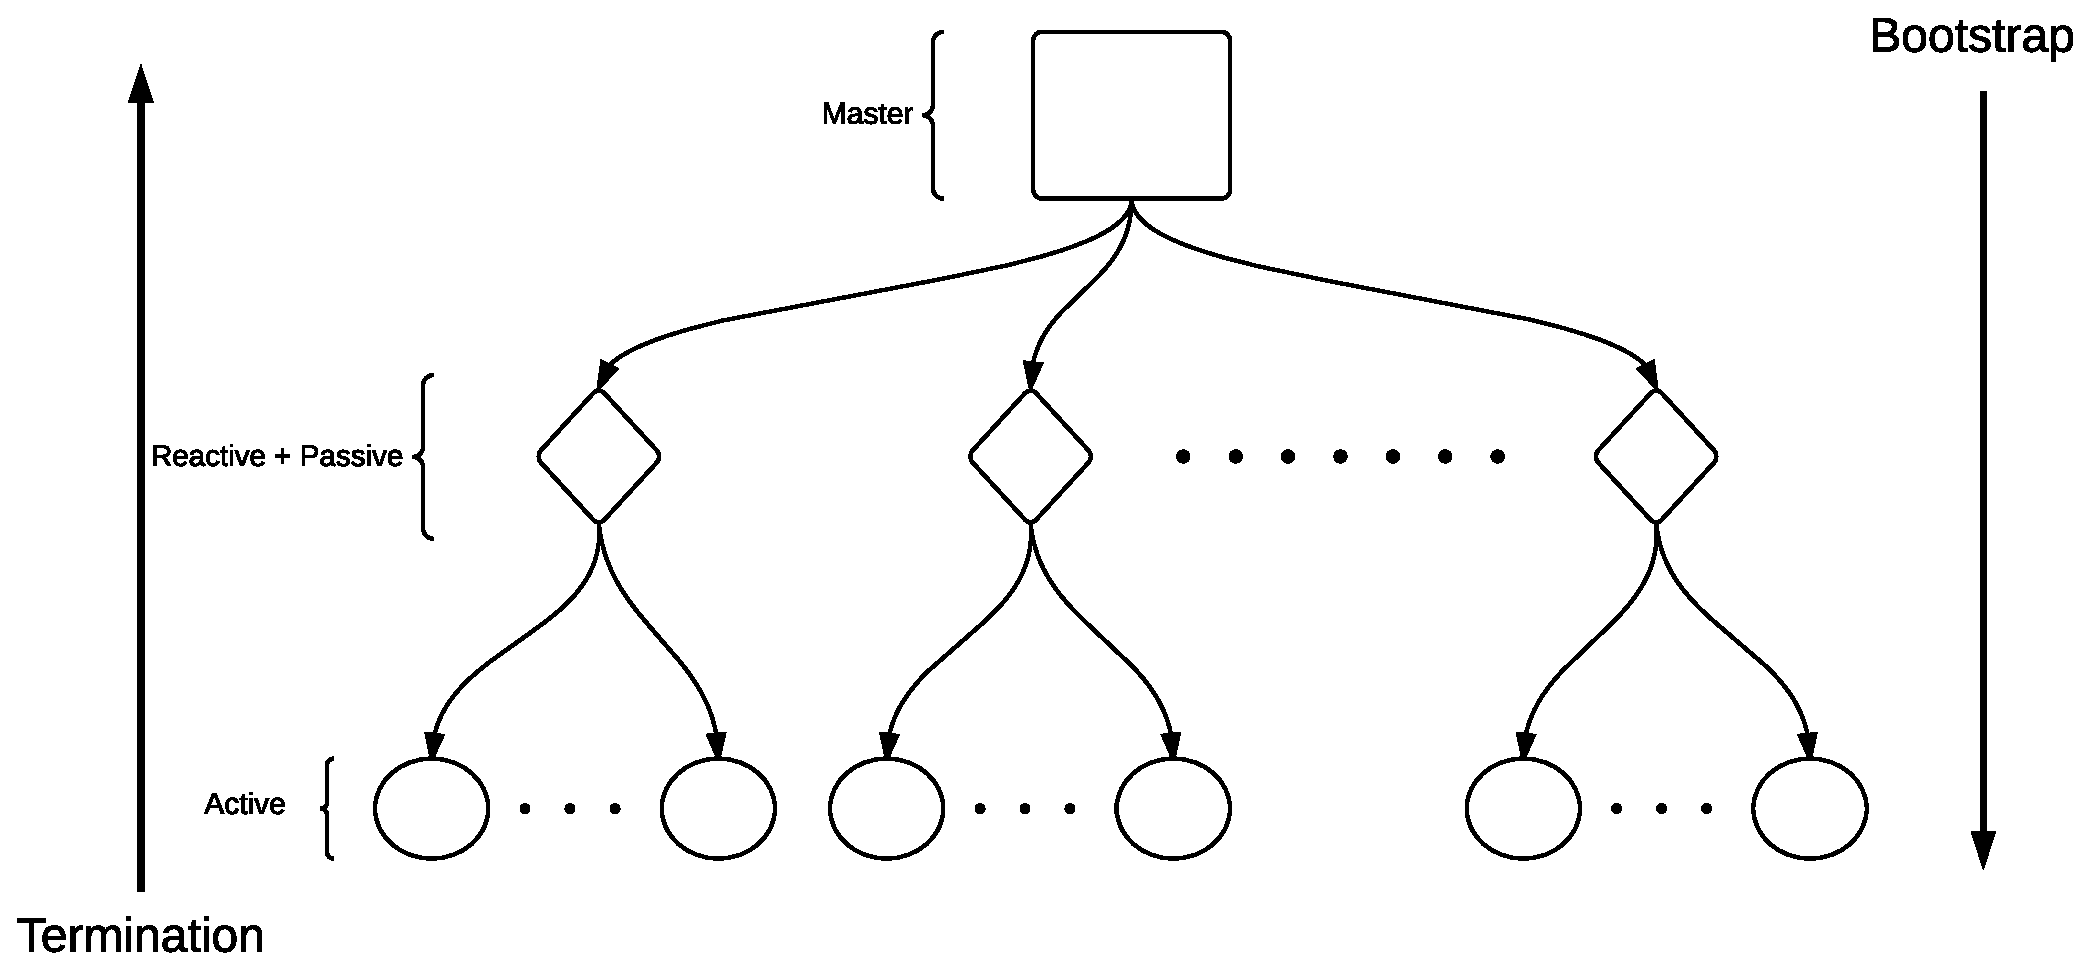
\includegraphics[width=\columnwidth]{images/solution/app_proc_tree.eps}
  \caption{Application process tree}
  \label{fig:app-proc-tree}
\end{figure}

At the end of the bootstrap, the \textit{Master} process has to notify the
middleware layer of the successful completion. A crash of the
\textit{Master} process, occurring before the end of the bootstrap,
is signaled to the middleware layer, by the expiration of a timeout bound to
the \texttt{app.boot} call.
Note that this model works also for a bootstrap which is executed starting
from a snapshot of the system, with the only difference consisting in divergent
values of the configuration file. Indeed, we have to use a set of
configurations, which is going to be different for each city.